\setcounter{rownumber}{0}
\chapter{Manuscript I: Laser cooling of traveling wave phonons in an optical fiber}
\label{ch:Cooling}
\acresetall

\textit{This chapter elaborates on experiments and results related to optomechanical cooling, which have been published as an article of the same name in Physical Review Applied by Johnson et al. (2023) \cite{johnson2023laser}. Any discrepancies, omissions, or errors that may exist between the published paper and this dissertation chapter are the sole responsibility of the author, as the text, analyses, and interpretations herein represent an independent and original presentation of the work.}

%--------------------------------------------------------------------%

\section{Introduction}
\label{sec:Cooling:Introduction}

Materials above the ground state experience therodynamic variations such as temperature and density. These thermal fluctuations alter the optical properties of a given material, allowing a scattering process to occur (see Section \ref{sec:Introduction:Light-Scattering}). Spontaneous Brillouin scattering is the inelastic scattering of light with these thermal fluctuations within a material, facilitating an energy exchange between the optical and acoustic domains. While a given medium typically supports a multitude of thermally excited acoustic modes (including both transverse and longitudinal modes) we focus here specifically on longitudinally travelling acoustic waves to demonstrate cooling in a continuous (non-resonant) system.

[lit review, state of the art]

%--------------------------------------------------------------------%

\section{Optomechanical Cooling and Heating}
\label{sec:Cooling:Cooling-Heating}

Backward Brillouin scattering targets longitudinally traveling acoustic waves (or phonons) through two complementary processes---Stokes and anti-Stokes, illustrated in Figures \ref{fig:Cooling:StokesHeating} and \ref{fig:Cooling:anti-StokesCooling}, respectively. In the Stokes process, an incident photon of frequency \(\omega\) scatters with a \textit{retreating} phonon of frequency \(\Omega\) annihilating the \textit{photon} and creating both an additional phonon of frequency \(\Omega\) and a backscattered photon at the difference energy (\(\omega_{\mathrm{Stokes}} = \omega - \Omega\)). In this way, both energy and momentum are conserved. This can be visualized by an analogy, in which the incident light experiences a doppler \textit{down}-shift in frequeny as though the photon were reflected from a retreating mirror. Since this processes results in an increase in the phonon population within the respective longitudinal mode of the material, this process is referred to as optomechanical heating. The energy lost by the light is gained by the material in the form of mechanical vibrations.

\begin{figure}[t]
    \centering
    \begin{subfigure}[b]{0.49\textwidth}
        \centering
        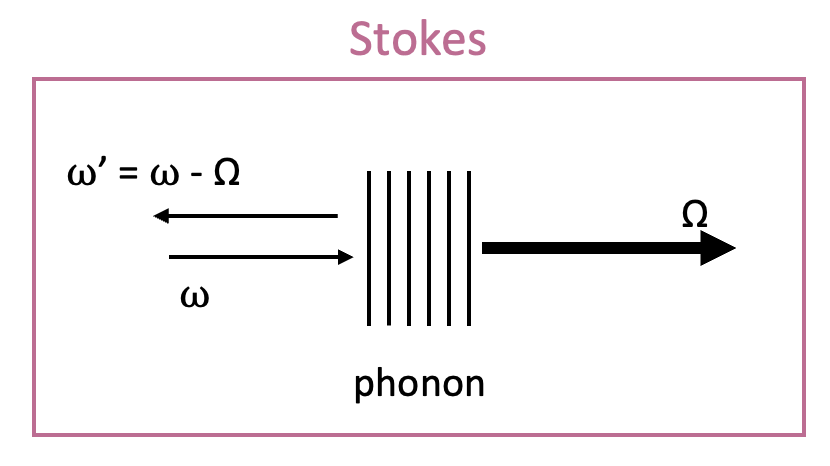
\includegraphics[width=\textwidth]{figs/3-Cooling/StokesHeatingProcess.png}
        \caption{}
        \label{fig:Cooling:StokesHeating}
    \end{subfigure}
    \hfill
    \begin{subfigure}[b]{0.49\textwidth}
        \centering
        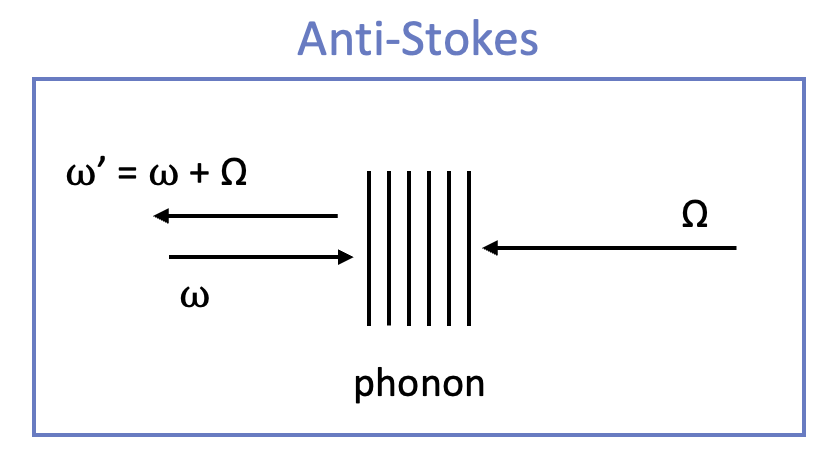
\includegraphics[width=\textwidth]{figs/3-Cooling/anti-StokesCoolingProcess.png}
        \caption{}
        \label{fig:Cooling:anti-StokesCooling}
    \end{subfigure}
    \caption{Illustration of optomechanical heating and cooling processes. Figure \ref{fig:Cooling:StokesHeating} shows an incident photon of frequency \(\omega\) scattering with a retreating phonon of frequency \(\Omega\), resulting in the annihilation of the incident photon and the creation of both an additional retreating phonon of frequency \(\Omega\) and a backwards propagating photon of reduced frequency and thereby energy (\(\omega_{\mathrm{Stokes}} = \omega - \Omega\)). Figure \ref{fig:Cooling:anti-StokesCooling} shows the inverse process, whereby an incident photon, \(\omega\), scatters with an approaching phonon, \(\Omega\), annihilating the incident photon and the phonon to produce a backwards propagating photon of increased frequency and thereby energy (\(\omega_{\mathrm{anti-Stokes}} = \omega + \Omega\)).}
    \label{fig:Cooling:StokesProcesses}
\end{figure}

The anti-Stokes process is the inverse process, whereby an \textit{approaching} phonon of frequency \(\Omega\) scatters with an incident photon of frequency \(\omega\), annihilating the \textit{phonon} and creating a backscattered photon at the addition energy (\(\omega_{\mathrm{anti-Stokes}} = \omega + \Omega\)). Both energy and momentum are again conserved, however in the anti-Stokes process, the incident light experiences a doppler \textit{up}-shift in frequency as if, to continue the analogy, the photon were reflected from an approaching mirror. For further intuition, one might consider an elastic collision of a ball (the photon) with a moving wall (the phonon) for the cases of the wall moving towards (in the anti-Stokes process) or away (in the Stokes process) from the ball as they collide. This simple analogy helps illustrate how momentum and energy are exchanged in optomechanical heating (Stokes) and cooling (anti-Stokes) processes.

While these processes naturally lead to a change in phonon population and thereby mode temperature, specific challenges arise in practical demonstration and detection of the phenomena. The most significant challenge is that since we are seeking to address the natural thermal phonons of the medium, we are restricted to a spontaneous Brillouin scattering regime as opposed to stimulated. Stimulated Brillouin scattering techniques are often employed to dramatically increase scattered power and aid in detection (see Appendix \ref{appendix:comparison} and specifically Figure \ref{fig:SponBSvsStimBSvsCoBS} for a comparison of scattered power produced by different Brillouin techniques). However, when stimulated conditions are met, the thermal phonons of the medium are actively driven, often by the injection of an additional optical field. Therefore, the stimulated scattering process is no longer a result of spontaneous thermal phonons but rather of optically driven phonon populations. As explained in Appendix \ref{appendix:comparison}, the condition for achieving stimulated Brillouin scattering is an overall process gain factor, \(G = G_{B}P_{P}L\), much greater than unity \((G \gg 1)\), where \(G_{B}\) is the effective Brillouin gain, \(P_{P}\) is the pump power, and \(L\) is the effective length. An ideal testbed for demonstrating optomechanical cooling would therefore feature an overall process gain factor near but not exceeding unity in order to maximize feasibility of measurement while ensuring a spontaneous scattering regime.

In addition to this fundamental requirement, rate conditions provide additional criticl constraints. The rate at which the phonons are depleted through the optomechanical cooling process must exceed the replenishment rate by the surrounding thermal bath.

Ideal testbed for demonstrating optomechanical cooling:
1) Large acousto-optic coupling
2) Tight confinement of light and sound
3) Sound speed not too fast (too large brillouin frequency shift, expensive fast elecronics for detection) or too slow (too small brillouin frequency shift, making it hard to separate sideband from carrier)
4) Large single pass gain GPL
5) Fast escape condition - phonon mode depletion rate must exceed repopulation rate 4vg/L > Gamma

%--------------------------------------------------------------------%

\section{Cooling Platform: \texorpdfstring{$CS_{2}$}{CS2}-Liquid Core Optical Fiber}
\label{sec:Cooling:Platform}

Demonstration of optomechanical cooling and heating of traveling wave phonons requires a device or material host that [can balance all of the requirements I just layed out in the previous section!] features large optomechanical coupling as well as tight optical and acoustic confinement for large acousto-optic overlap.  a \ce{CS2}-filled \ac{LCOF} similar to that used by Behunin et al. (2019). \cite{behunin2019spontaneous}

\subsection{Optomechanical Properties}
\label{subsec:Cooling:Platform:Properties}


\section{Fabrication of \texorpdfstring{$CS_{2}$}{CS2}-Liquid Core Optical Fiber}
\label{subsec:Cooling:Platform:Fabrication}

The fabrication process for the \ce{CS2}-\ac{LCOF} involved several key steps for each of the two ends: splicing \ac{SMF-28} to \ac{UHNA7} fiber, preparing and angle-cleaving fibers, cutting and preparing a protective glass vial, and finally securing the assembly on a microscope slide. Figure \ref{} illustrates the overall schematic of the fiber fusion strategy, showing how \ac{SMF-28} and \ac{UHNA7} fibers flank the hollow core. The following sections detail each step in the fabrication protocol.

\subsection{Splicing \ac{SMF-28} to \ac{UHNA7}}

Before integrating the hollow-core segment, a segment of Corning \ac{SMF-28} was spliced to Thorlabs \ac{UHNA7} fiber. This transition was necessary to gradually match the mode fields and reduce losses at the interface with the hollow-core region.

To begin, a short length (\SI{0.5}{\meter}) of \ac{SMF-28} was stripped, cleaved flat, and fusion-spliced to 5–\SI{10}{\centi\meter} of similarly prepared \ac{UHNA7} fiber. The initial splice was performed with standard parameters, but the arc was then repeated four to five times under carefully moderated power. This multiple-arc “tapering” approach helped narrow the \ac{SMF-28} core (\SI{9.2}{\micro\meter} diameter) where it contacted the smaller \ac{UHNA7} core (\SI{2.4}{\micro\meter} diameter), improving coupling efficiency. Prior to and following the splice, optical transmission measurements were taken to assess the splice quality.

\subsection{Preparing the \ac{UHNA7} Fiber}

After the preliminary \ac{SMF-28}–\ac{UHNA7} splice, the \ac{UHNA7} fiber needed to be angle-cleaved to interface properly with the hollow-core segment. An angle-cleaver with a built-in vacuum mechanism was used for this process:

\begin{enumerate}
	\item Equipment Setup: The angle-cleaver and its vacuum pump were turned on, and the cleaver’s dedicated software interface was opened. Approximately two minutes was allowed for the vacuum level to stabilize.
	\item Fiber Positioning: The left fiber clamp block was pivoted fully to the left, and the \ac{UHNA7} fiber was placed so that its freshly cleaved tip was centered over the reference circle at the splice head.
	\item Alignment: While the vacuum held the fiber in place, the cleaver’s camera view was used to align the sharpest angle of the \ac{UHNA7}’s end face to ensure a precise angular cleave. A small “flag”—a piece of unstripped fiber taped on top of the \ac{UHNA7}—was sometimes used to help the clamp grip consistently.
	\item Pivot and Support: The left block was pivoted back and forth until the \ac{UHNA7} tip was near the correct horizontal position. A folded piece of support paper and two boxes of Kimtech Kimwipes on the benchtop were used to prevent the fiber from drooping and to minimize the risk of cracking or breakage during handling.
\end{enumerate}

\subsection{Preparing the Hollow-Core Fiber}

Once the \ac{UHNA7} fiber was properly angle-cleaved, the hollow-core fiber segment was prepared for splicing:

\begin{enumerate}
	\item Stripping and Cleaving: The hollow-core fiber coating was gently dissolved in acetone and wiped away to expose the bare glass. It was then cleaved flat rather than at an angle.
	\item Positioning on the Cleaver: The right clamp block was pivoted to its stop position, and the hollow-core fiber was placed so its end was centered over the splice head’s circle, ensuring no physical contact with the \ac{UHNA7} fiber.
	\item Flag and Alignment: As with the \ac{UHNA7}, a flag of unstripped fiber was placed above the hollow-core fiber to facilitate stable clamping. The right clamp block was slowly pivoted toward the center until the fiber tips were close but still not touching. Like before, the fiber was supported with paper and Kimwipe boxes to prevent bending.
\end{enumerate}

\subsection{Cleaning and Preparing the Microscope Slide}

Because the final splice assembly must be encapsulated for protection, it was mounted on a clean microscope slide. The slide was scrubbed with soap and a soft toothbrush under running hot water, then thoroughly rinsed and dried with an air gun. Clean handling was crucial, so the slide was placed inside a folded Kimwipe for safekeeping until needed.

\subsection{Cutting and Preparing the Glass Vial}

A small glass vial was used to form a protective enclosure over the splice region and allow liquid to fill the hollow core.

\begin{enumerate}
	\item Cutting the Vial: Wearing gloves and safety glasses, a new glass vial was secured carefully by hand and cut at low rotational speed on a saw. The cut removed only the bottom portion of the vial so that the main body of the vial remained relatively long.
	\item Flattening and Notching: The cut edge was smoothed and flattened with a file block, and two shallow, wide straddle-gaps were added on opposite sides of the new opening. These gaps would later accommodate the fiber on the slide. Ensuring these gaps were shallow aided subsequent epoxy sealing, while making them wide reduced the risk of inadvertently contacting and damaging the delicate splice during vial placement.
	\item Cleaning: Finally, the vial was scrubbed with dish soap and a pipe cleaner, rinsed, dried with compressed air, and recapped until needed.
\end{enumerate}

\subsection{Angle-Splicing the \ac{UHNA7} to the Hollow-Core Fiber}

The next step was to form the final angle splice between the \ac{UHNA7} fiber and the hollow-core segment within the fusion splicer:

\begin{enumerate}
	\item Positioning and Auto-Alignment: With both fibers supported and extending naturally from opposite blocks, the splicer’s auto-alignment was initiated. The system brought the fibers within viewing distance so the operator could adjust vertical and horizontal positioning.
	\item Core Alignment: Using the splicer’s camera interface, the UHNA7 core was lined up with the hollow-core’s central region. Small vertical and horizontal translations ensured good overlap.
	\item iber Touch-Off: The left fiber (\ac{UHNA7} side) was carefully advanced until the tips touched, then retracted slightly to avoid excessive bending or damage.
	\item Argon Gas Flow and Arc: An argon flow was introduced to shield the fusion region from contaminants, and the fusion arc was applied. Images were taken at each step to verify the splice quality. If alignment or splicing was inadequate, the fibers were separated, re-cleaved if necessary, and the procedure repeated. After confirming a good splice, the argon was turned off and the splicer was shut down.
\end{enumerate}

\subsection{Transferring the Spliced Fibers onto the Slide}

Upon completing the angle splice, the fiber assembly needed to be moved gently off the splicer onto the prepared microscope slide:

\begin{enumerate}
	\item Release and Stabilization: With the splicer’s vacuum pump turned off, the fiber typically lifted out of the groove as the vacuum seal broke. Tweezers were used to remove any fiber “flags,” and wooden craft sticks helped lift the fibers from the block grooves without sharp bends.
	\item Placement on the Slide: The slide was positioned in front of the splicer head, and the fibers were transferred carefully in a smooth motion. Two small drops of epoxy were placed on each side of the splice region to tack the fiber down. This was allowed to cure for at least five minutes.
\end{enumerate}

\subsection{Enclosing the Splice with the Cut Vial}

The splice region was enclosed in a glass vial to protect the hollow-core’s interior and to facilitate later filling with liquid:

\begin{enumerate}
	\item Positioning the Vial: The prepared vial was placed over the splice region by sliding one straddle-gap around the fiber first, then tilting it so the second gap aligned. Gloves were worn to prevent transferring skin oils onto the vial.
	\item Epoxy Sealing: A fresh mixture of two-part epoxy was prepared in roughly equal proportions and thoroughly mixed for 10–15 seconds to ensure a uniform bond. Generous epoxy was applied around the vial’s perimeter where it contacted the slide. Care was taken to avoid epoxy wicking into the splice itself. The assembly was then left undisturbed for at least five minutes to cure.
\end{enumerate}

\subsection{Final Mounting and Labeling}

Once the epoxy had set, the slide was labeled with the date, splice reference, and relevant notes using a marker. For long-term handling, the slide and its fibers were taped to a foam board or a similarly stable surface to prevent accidental jostling. This procedure ensured a robust, low-loss transition from \ac{SMF-28} to \ac{UHNA7} to the hollow-core fiber. The careful cleaning steps, controlled splicing environment with argon shielding, and meticulous handling minimized the risk of fiber breakage and guaranteed a clean optical interface. Encapsulating the splice with a modified glass vial on a microscope slide allowed easy manipulation of the hollow core’s environment, which was crucial for subsequent liquid filling and optical characterization experiments.

Finally, this entire procedure must be repeated on the opposite side of the hollow-core fiber to complete the \ac{LCOF} assembly. Each splice should be robust enough to guide light but also “broken” sufficiently to allow \ce{CS2} to enter the hollow core via capillary action in the next step.


\subsection{Fabrication Iterative Refinement}
\label{subsec:Cooling:Platform:Refinement}

%--------------------------------------------------------------------%

\section{Intention of the Pump-Probe Experiment}
\label{sec:Cooling:Intention}

%--------------------------------------------------------------------%

\section{Experimental Setup}
\label{sec:Cooling:Setup}


\subsection{Main Experiment}
\label{subsec:Cooling:Setup:Main}


\subsection{Pump-Probe Experiment}
\label{subsec:Cooling:Setup:Pump-Probe}

%--------------------------------------------------------------------%

\section{Results}
\label{sec:Cooling:Results}


\subsection{Main Experiment Results}
\label{subsec:Cooling:Results:Main}

need for normalized cooling metric - per pump power, and such that one cannot start a system in a heated state to achieve a greater stated cooling ability. Or maybe room temperature is identical across systems? check. if not, normalize.

\subsection{Pump-Probe Experiment Results}
\label{subsec:Cooling:Results:Pump-Probe}

%--------------------------------------------------------------------%

\section{Discussion}
\label{sec:Cooling:Discussion}

Ideas to achieve net cooling, one might design a system where:

1) single pass gain bias
     swing energy transfer bias to favor anti-Stokes over Stokes (mode-dependent gain)
     the Stokes process were not permitted (ryan's only idea), or just significantly restricted - what is that bias threshold requirement?
     currently, we are net *heating* the system because it is easier to heat from equilibrium than cool (right? explore this. it's also hard to make it hotter beyond a certain point.)
     implementation ideas:
       multi-pump scheme to destructively interfere with Stokes and/or constructively interfere with anti-Stokes
       doping or specialized waveguide gratings that pick out the Stokes band for out-of-plane scattering

2) time bias
     create an energy transfer *rate* bias between Stokes and anti-Stokes
     can be accomplished with either the brillouin energy transfer rate or the repopulation rate

       brillouin process rate:
         4vg/L, have either group velocity or length be different for Stokes vs anti-Stokes (smaller vg or larger L for Stokes than anti-Stokes)
         make anti-Stokes fast light and/or Stokes slow light
         vg inversely proportional to pump power, so it's a balance
           increasing pump power = slower escape time (4vgL), and also larger dissipation (Gamma+)

       repopulation rate:
         thermally insulate the anti-Stokes mode from the thermal bath that would repopulate it
         or at least insulate it some amount more than Stokes (what is that threshold? even if it's only net cooled for picoseconds, what is that minimum crossover point insulation bias point)
         essentially locks in the cooled mode while letting the heated mode spill out
         implementation idea:
           design a fiber/waveguide with acoustic directional bias, such that phonons travelling one direction dissipate quicker because of the geometry/acoustic properties of the fiber. (triangles? acting as tapered acoustic dissipators, pointing in one direction?)

3) starting temperature
     Could you acieve net cooling in a cheap and dirty sense by starting the system in a very heated state, thus invoking a natural dissipation rate bias?! - yes!
     Things do naturally run hot, perhaps no extra fancy engineering is needed for some practical systems? (data processing, reduce thermal noise from above ambient heat)
     not traditional definition of optical refrigeration below ambient/thermal bath, but still *useful*
     is this already done? lit search

Think about a practical device or system for each of these cases (think waveguide playground!)

\subsection{Application to Ground State Cooling}
\label{subsec:Cooling:Discussion:Ground-State}


\subsection{Standardized Cooling Metric}
\label{subsec:Cooling:Discussion:Metric}


\subsection{Tapered chalcogenide Photonic Crystal Fiber: Max Plank Results}
\label{subsec:Cooling:Discussion:Max-Plank}
